\documentclass[10pt,oneside,swedish]{lips_no-customer}

%\usepackage[square]{natbib}\bibliographystyle{plainnat}\setcitestyle{numbers}
\usepackage[round]{natbib}\bibliographystyle{plainnat}

% Configure the document
\title{Generell mall}
\author{Redaktör namn}
\date{1 november 2016}
\version{1.0}

\reviewed{ReviewerName}{2015-xx-xx}
\approved{ApproverName}{2015-xx-xx}

\projecttitle{En inspirerande titel}

\groupname{Gruppnamn}
\groupemail{groupmail@liu.se}
\groupwww{http://www.isy.liu.se/tsrt10/group}

\coursecode{TSRT10}
\coursename{Reglerteknisk projektkurs}

\orderer{Beställare, Linköpings universitet}
\ordererphone{+46 xxxxxx}
\ordereremail{ordere@liu.se}

% \customer{Kund, Företag X}
% \customerphone{+46 xxxxxx}
% \customeremail{customer@companyx.com}

\courseresponsible{Boss Person}
\courseresponsiblephone{+46 xxxxxx}
\courseresponsibleemail{the.boss@liu.se}

\supervisor{Handledare}
\supervisorphone{+46 xxxxxx}
\supervisoremail{super.visor@liu.se}

\smalllogo{logo} % Page header logo, filename
\biglogo{logo} % Front page logo, filename

\cfoot{\thepage}
\begin{document}
\maketitle

\cleardoublepage
\makeprojectid

\cleardoublepage
\tableofcontents

\cleardoublepage
\section*{Dokumenthistorik}
\begin{tabular}{p{.06\textwidth}|p{.1\textwidth}|p{.45\textwidth}|p{.13\textwidth}|p{.13\textwidth}} 
  \multicolumn{1}{c}{\bfseries Version} & 
  \multicolumn{1}{|c}{\bfseries Datum} & 
  \multicolumn{1}{|c}{\bfseries Utförda förändringar} & 
  \multicolumn{1}{|c}{\bfseries Utförda av} & 
  \multicolumn{1}{|c}{\bfseries Granskad}\\
  \hline
  \hline
  0.1 & 2019-10-07 & Första utkast & & \\
  \hline
\end{tabular}

\cleardoublepage
\pagenumbering{arabic}\cfoot{\thepage}

\section{Syfte och mål}

Syftet med projektet är att konstruera ett system som kör bilar att runt en
bilbana. Till bilbanan finns det 9 ``givare'' som när de passeras skickar en
signal. Med hjälp av tidsskillnaden mellan signalerna kan man räkna ut hur lång
tid det tog för en bil att åka mellan två givar. Bilbanan är även kopplad till
en dator där det finns möjlighet att justera bilarnas gaspådrag med en
spänningstillförsel. Med hjälp av denna information ska ett system skapas som
kör en eller två bilar runt bilbanan på en inställbar varvtid mellan 12 och 15
sekunder, samt gör att bilarna åker i mål så nära varandra i tiden som möjligt.

\section{Delsystem}

\input{system/bana}
\section{Display}

När programmet startas visar displayen möjligheten att välja aktiv bana, om
gemensam målgång ska vara aktiverad, vilken varvtid bilarna ska hålla och
eventuellt hur många varv bilarna ska köra runt banan (exkluderat de fem
kalibreringsvarven). Se figur~\ref{fig:disp:before}.

Under körning ska displayen för varje bil visa den förra varvtiden, hur många
varv bilen kört, nuvarande hastighet och pålagd spänning. Användaren kan också
trycka på en knapp för att avbryta körningen. Se figur~\ref{fig:disp:during}. I
mån av tid ska displayen även visa en karta över banan och var systemet tror
att bilarna befinner sig.

Efter körningen är avklarad ska displayen visa olika grafer. Enligt
kravspecifikationen ska varvtid per varv och snitthastigheten för varje segment
visas enligt figur~\ref{fig:disp:after}. I mån av tid ska endast en graf åt
gången visas på skärmen och användaren ska kunna välja vilken graf som ska
visas med hjälp av tryckbara knappar längst upp på skärmen.

\begin{figure}
  \centering
  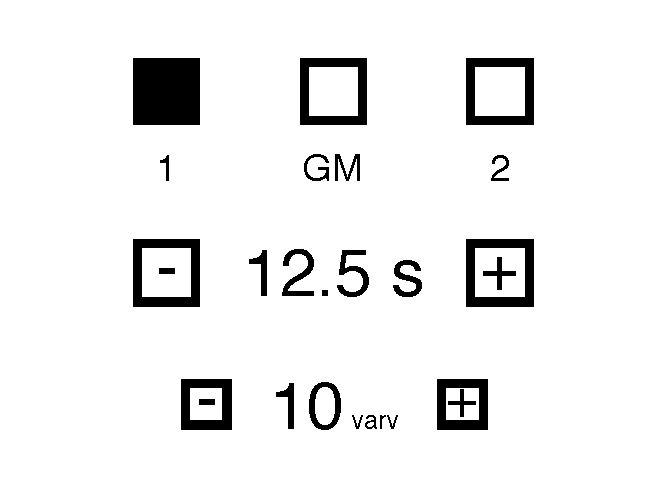
\includegraphics{figures/innan}
  \caption{Displayens utseende vid val av körinställningar.}
  \label{fig:disp:before}
\end{figure}
\begin{figure}
  \centering
  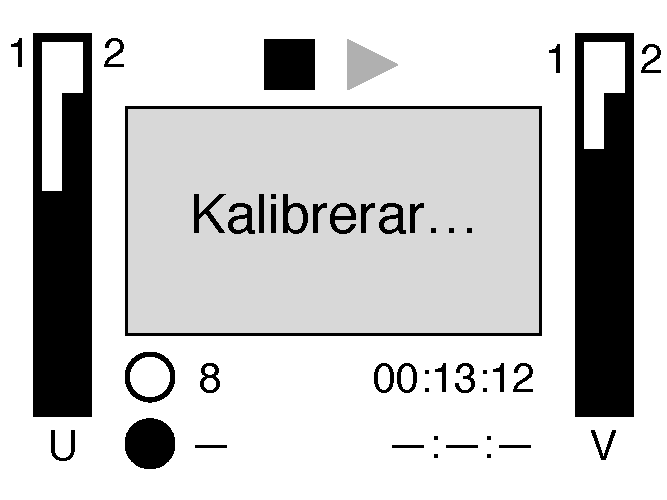
\includegraphics{figures/under}
  \caption{Displayens utseende under körning.}
  \label{fig:disp:during}
\end{figure}
\begin{figure}
  \centering
  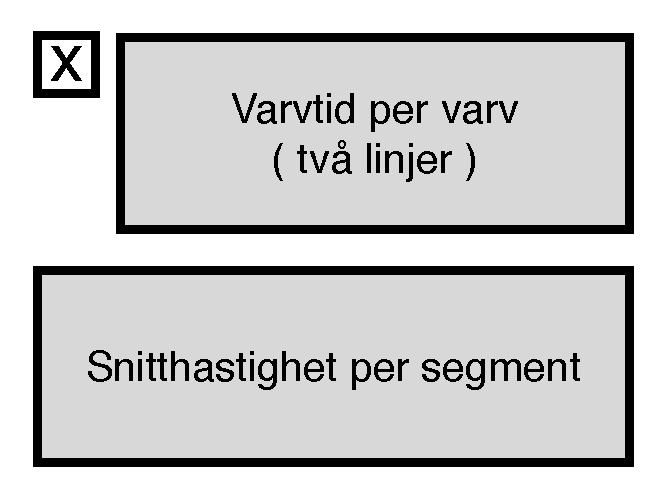
\includegraphics{figures/efter}
  \caption{Displayens utseende när körning är avklarad.}
  \label{fig:disp:after}
\end{figure}


Programmet ska detektera att en bil har åkt av banan inom 10 sekunder. Detta
ska göras genom att felvarna, avbryta programmet och skriva ut detta på
displayen om programmet inte registrerar en ny givare inom dessa tio sekunder.


\end{document}

%%% Local Variables:
%%% mode: latex
%%% TeX-master: t
%%% End:
